\documentclass[a4paper, 12pt]{article}
\usepackage[english]{babel}
\usepackage[pdftex]{graphicx}
\usepackage[T1]{fontenc}
\usepackage{wrapfig}
\usepackage{graphicx} 
\usepackage{algorithm}
\usepackage{hyperref}
\usepackage{amssymb}
\usepackage{biblatex} 
\addbibresource{Citations.bib}
\usepackage{csquotes}

\newcommand{\HRule}{\rule{\linewidth}{0.3mm}}

\begin{document}
\begin{center}
% Title
\HRule \\[0.3cm]
{ \LARGE \bfseries Internship first week report \\[0.3cm]}
{ \LARGE \bfseries 30/06/25 - 04/07/25 \\[0.1cm]}
\HRule \\[1.5cm]

% Author and supervisor
\begin{minipage}[t]{0.45\textwidth}
\begin{flushleft} \large
\textsc{supervisors :}\\
Bruno \textsc{Quoitin}\\
Aqeel \textsc{Ahmed}\\
\end{flushleft}

\end{minipage}
\begin{minipage}[t]{0.45\textwidth}
\begin{flushright} \large
\textsc{author :}\\
Maxime \textsc{Bartha}\\
\end{flushright}
\end{minipage}\\[2ex]
\end{center}

Explain the TCP IP conn between Rx and Tx, explain Arduino code, 

explain the sync



\section{Initial objectives}
My initial objectives during this first week were to :
\begin{itemize}
  \item set the goals for the internship
  \item look at what as been done last year in details
  \item decide on what to work on
\end{itemize}


Last year, the method to capture LoRa frames was to detect them by implementing an algorithm found in \cite{demToDec}.

This year, we decided that I will be implementing a time synchronisation method to classify the captures of LoRa frames.

\section{Material and software used}
Material :
\begin{itemize}
  \item sdr : pluto, usrp, rtl
  \item arduino MKR1310
\end{itemize}
Software : 
\begin{itemize}
  \item gnu radio companion : a block based programming software for signal processing.
  \item inspectrum : an open source spectrogram

\end{itemize}

\section{Summary}
I've managed to implement a proof of concept of the time synchronisation method explained in section \ref{TSi}.
I've learned about TCP socket connections, Serial Arduino communication and gnu radio programming.

\section{Time synchronisation implementation} \label{TSi}
There is basically 3 parts to this implementation: 
\begin{itemize}
  \item The receiver side capturing the LoRa frames
  \item The transmitter side in charge of controlling which device should transmit
  \item The Arduino implementation handling the transmission
\end{itemize}

The transmitter is in charge of taking all the transmission parameters such as frequency, bandwidth, spreading factor, number of frames to transmit per devices (cycles) and synchronisation parameters such as phase and period.

The receiver is in charge of capturing the LoRa frames and classify them by device.

The arduino devices transmit LoRa frames when the transmitter tells them to.

\vspace{1cm}

\subsection{Transmitter-arduino relation}
Let's first take a look at the relation between the transmitter and the arduino devices :

Its first job is to communicate all the thransmission parameters to all the arduino devices connected to it by sending an InitFlag followed by the parameters. 

Then the when an arduino is initiated, it waits for a SendFlag for it to transmit a single LoRa frame. After Sending it, the arduino goes back to waiting for a SendFlag until it sent all the frames it had to.

A state machine showing this relation can be found in the figure \ref{ardSM}.

\begin{figure}
  \begin{center}
    \includegraphics[width=0.7\textwidth]{images/arduinoStateMachine.jpg}
  \end{center}
  \caption{arduino state machine}\label{ardSM}
\end{figure}


\subsection{Transmitter-receiver relation}
First, the receiver sets itself as a socket server on a certain port. The transmitter connects to this socket using the port and the receiver's IP address. Then when the connection is done, the transmitter sends all the synchronisation parameters to the receiver such as : 
\begin{itemize}
  \item the starting transmission time in absolute time minus half a period 
  \item a list of the devices ordered by device id
  \item the period between each transmission
\end{itemize}

Then on both sides, after the starting time is reached, the transmitter sends LoRa frames each period and the receiver saves each capture based on the device id.

To know which device is currently sending, the frames are sent by cycling through the device id list.

\subsection{Saving structure}
A saving directory and scenario name have to be given. 
The structure can be seen in figure \ref{savestruct}

\begin{figure}[H]
  \begin{center}
    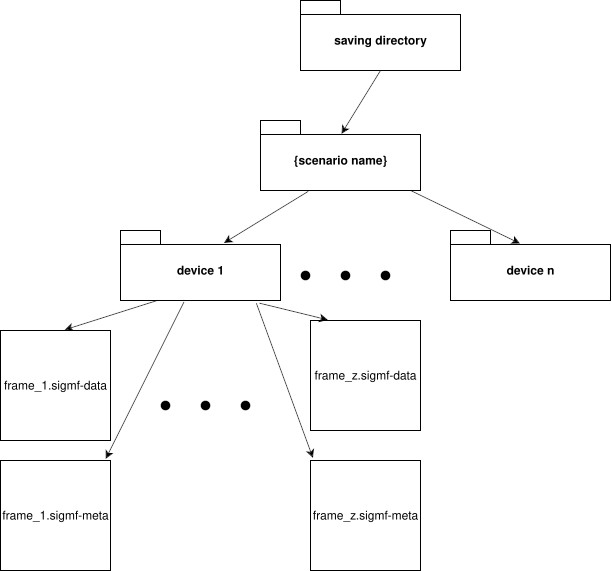
\includegraphics[width=0.6\textwidth]{images/save.jpg}
  \end{center}
  \caption{saving structure}\label{savestruct}
\end{figure}

Each .sigmf-meta files contains :
\begin{itemize}
  \item the data type (c32\_le)
  \item the frequency
  \item the sample rate
  \item the capture time
  \item a description taking the distance, outdoor/indoor and other possible parameters
\end{itemize}

\subsection{Improvements}
Some improvements can be made in this implementation :
\begin{itemize}
  \item use implicit header for the LoRa frame
  \item check when receiving a frame that the expected device id is the device id sent in the frame (needs decoding)
  \item make the arduino state machine and the error handling more robust  
\end{itemize}

\section{Problems encountered} 
Serial ports issues when connecting certain devices

\section{Conclusion}
In conclusion, the implementation of the time based synchronisation is not yet robust and still needs some attention.
The most important aspect is "is the data collected reliable". It's the main question I will be trying to answer in the second week.

\printbibliography

\end{document}
